%%%%%%%%%%%%%%%%%%%%%%%%%%%%%%%%%%%%%%%%%%%%%%%%%%%%%%%%%%%%%%%%%%%%%%%%%%%%%%%%%%%%%%%%
% Beamer LaTeX template
%
% Version 1.0.0 (17/02/2023) [dd/mm/aaaa]
%
% Original author: Jesper Kjær Nielsen, Aalborg University, Denmark
% Original template: aalborg-university-beamer-theme
%
% Modified by: Alberto Cuadra-Lara (acuadra@ing.uc3m.es) | acuadralara.com
%
% License: GPLv3 (https://www.gnu.org/licenses/gpl-3.0.html)
%%%%%%%%%%%%%%%%%%%%%%%%%%%%%%%%%%%%%%%%%%%%%%%%%%%%%%%%%%%%%%%%%%%%%%%%%%%%%%%%%%%%%%%%

%%%%%%%%%%%%%%%%%%%%%%%%%%%%%%%%%%%%%%%%%%%%%%%%%%%%%%%%%%%%%%%%%%%%%%%%%%%%%%%%%%%%%%%%
% Document setup and packages
%%%%%%%%%%%%%%%%%%%%%%%%%%%%%%%%%%%%%%%%%%%%%%%%%%%%%%%%%%%%%%%%%%%%%%%%%%%%%%%%%%%%%%%%
% Set document class: font size, aspectratio (e.g., 1609 or 1610)
\documentclass[9pt, aspectratio=1609]{beamer}

% Setup theme
\usetheme[
%%% options passed to the outer theme
%    hidetitle,           % hide the (short) title in the sidebar
%    hideauthor,          % hide the (short) author in the sidebar
%    hideinstitute,       % hide the (short) institute in the bottom of the sidebar
%    shownavsym,          % show the navigation symbols
%    width=2cm,           % width of the sidebar (default is 2 cm)
%    hideothersubsections,% hide all subsections but the subsections in the current section
%    hideallsubsections,  % hide all subsections
%    left                 % right of left position of sidebar (default is right)
  ]{Aalborg}
  
% Comment: if you want to change the colors of the various elements in the theme, edit and uncomment the following lines

% * Change the bar and sidebar colors:
%\setbeamercolor{Aalborg}{fg=red!20,bg=red}
%\setbeamercolor{sidebar}{bg=red!20}
% * Change the color of the structural elements:
%\setbeamercolor{structure}{fg=red}
% * Change the frame title text color:
%\setbeamercolor{frametitle}{fg=blue}
% * Change the normal text color background:
%\setbeamercolor{normal text}{bg=gray!10}

% ... and you can of course change a lot more - see the beamer user manual.

% Set fontsizes
\setbeamerfont{footnote}{size=\tiny}
\setbeamerfont{caption}{size=\footnotesize}

% Load packages
\setbeamertemplate{caption}[numbered]
\usepackage[utf8]{inputenc}
\usepackage[english]{babel}
\usepackage[T1]{fontenc}
\usefonttheme{professionalfonts}
\usepackage{bm}
\usepackage{booktabs}
\usepackage{tikz}
\usepackage{hyperref}
\usepackage{fontawesome5}
\usepackage{academicons}
\usepackage{graphicx} 
\usepackage{xcolor} 
\usepackage{helvet}
\usepackage{multicol}
\usepackage{amsmath}
\usepackage{mathtools}
\usepackage{flushend}
\usepackage{cancel}
\usepackage{animate}
\usepackage{adjustbox}
\usepackage[version=3,arrows=pgf-filled]{mhchem}
\usepackage{pgfplots}

% Colors | rgb (from 0 to 1) | RGB (from 1 to 255)
\definecolor{applegreen}{rgb}{0.55, 0.71, 0.0}
\definecolor{myred}{rgb}{0.86,0.27, 0.3}
\definecolor{OrangeInks}{rgb}{1.0, 0.67, 0}
\definecolor{BlueInks}{rgb}{0, 0.67, 1.0}
\definecolor{BlackInks}{rgb}{0, 0, 0}
\definecolor{WhiteInks}{rgb}{1, 1, 1}
\definecolor{RedInks}{rgb}{1, 0, 0}
\definecolor{BlueInks2}{rgb}{0, 0.5, 0.8}
\definecolor{red}{rgb}{0.5765,0.0902,0.1765}
\definecolor{mygreen}{RGB}{28,172,0}
\definecolor{mylilas}{RGB}{170,55,241}
\definecolor{dkgreen}{rgb}{0,0.6,0}
\definecolor{gray}{rgb}{0.5,0.5,0.5}
\definecolor{mauve}{rgb}{0.58,0,0.82}
\definecolor{BoxCol}{rgb}{0.4471,0.6235,0.8118}
\definecolor{myblue}{RGB}{2, 147, 183}
\definecolor{mydblue}{RGB}{33,26,82}
\definecolor{myblue3}{RGB}{215, 213, 223}
\definecolor{myblue2}{RGB}{225, 230, 240}
\definecolor{cardinalred}{RGB}{184, 58, 75}
\definecolor{myorange}{RGB}{255, 175, 66}
\definecolor{greenstanford}{RGB}{0, 110, 81}
\definecolor{greensfmc}{RGB}{56, 122, 102}
\definecolor{redsfmc}{RGB}{156, 61, 43}
\definecolor{graytext}{RGB}{84,97,110}
\definecolor{mycolorbox}{rgb}{0.122, 0.435, 0.698}

% Define colors commands
\newcommand{\colorgreen}[1]{{\color{greensfmc}{#1}}}
\newcommand{\colorred}[1]{{\color{redsfmc}{#1}}}
\newcommand{\ch}[1]{{\color{myred}{#1}}}
\newcommand{\rev}[2]{{\color{BlueInks2}{\sout{#1}}\ \color{GreenInks}{#2}}}
\newcommand{\ac}[1]{{\color{cardinalred}{\textbf{#1}}}}
\newcommand{\acl}[1]{{\color{cardinalred}{#1}}}
\newcommand{\acll}[1]{{\color{myorange}{#1}}}
\newcommand{\aclgreen}[1]{{\color{greenstanford!55!white}{#1}}}
\newcommand{\chref}[2]{\href{#1}{{\usebeamercolor[bg]{Aalborg}#2}}}

% Define theme colors
\setbeamercolor{palette sidebar primary}{fg=mydblue}
\setbeamercolor{palette sidebar secondary}{fg=myblue2}
\setbeamercolor{palette sidebar tertiary}{fg=myblue2}
\setbeamercolor{palette sidebar quaternary}{fg=myblue2}
\setbeamertemplate{itemize items}[circle]

% Command to generate a text bullet as in itemize
\newcommand{\tabitem}{~~\llap{\textbullet}~~}

% To create boxes with colors
\usepackage[framemethod=tikz]{mdframed}
\usepackage{tcolorbox}
\newtcolorbox{mybox}{colback=mydblue!5!white,colframe=mydblue}

% Examples of the commands required to draw lines with the same colors as in the figure
\newcommand{\blackline}{\raisebox{2pt}{\tikz{\draw[-,BlackInks,solid,line width = 0.9pt](0,0) -- (5mm,0);}}}
\newcommand{\orangeline}{\raisebox{2pt}{\tikz{\draw[-,OrangeInks,solid,line width = 0.9pt](0,0) -- (5mm,0);}}}
\newcommand{\blueline}{\raisebox{2pt}{\tikz{\draw[-,BlueInks,solid,line width = 0.9pt](0,0) -- (5mm,0);}}}
\newcommand{\greenline}{\raisebox{2pt}{\tikz{\draw[-,GreenInks,solid,line width = 0.9pt](0,0) -- (5mm,0);}}}
\newrobustcmd*{\blankcircle}[1]{\tikz{\draw[draw=#1,line width = 0.9pt] (1mm,0) circle [radius=0.065cm];}}

% Settings tikz and pgfplot packages
\usetikzlibrary{arrows,decorations.pathmorphing,backgrounds,positioning,fit,petri,shadings,patterns,intersections}
\usetikzlibrary{external}
\pgfplotsset{compat=1.17}
\usepgfplotslibrary{fillbetween}

%%%%%%%%%%%%%%%%%%%%%%%%%%%%%%%%%%%%%%%%%%%%%%%%%%%%%%%%%%%%%%%%%%%%%%%%%%%%%%%%%%%%%%%%
% Define title, authors, affiliations, and logos
%%%%%%%%%%%%%%%%%%%%%%%%%%%%%%%%%%%%%%%%%%%%%%%%%%%%%%%%%%%%%%%%%%%%%%%%%%%%%%%%%%%%%%%%

% Define title
\title[
    % Optional (for long paper titles): title in the sidebar
    Linear Theory of Hypersonic Shocks Interacting with Turbulence in Air]{
    % Title in the titlepage
    \huge Linear Theory of Hypersonic Shocks\\[2mm] Interacting with Turbulence in Air
    }
    
% Define subtitle
% \subtitle{\small \textbf{1\textsuperscript{st}} Congress in ...}

% Define authors
\author[
    % Optional: authors in the sidebar
    \href{https://acuadralara.com}{A. Cuadra (presenter)}\\      
    \href{http://fluidosuc3m.es/people/mvcoello/}{M. Vera},
    \href{https://scholar.google.it/citations?user=jwcooaAAAAAJ&hl=en}{M. Di Renzo},
    \href{http://fluidosuc3m.es/people/chuete/}{C. Huete}]
{ 
    % Authors titlepage
    \textcolor{white}{\href{https://acuadralara.com}{\underline{Alberto Cuadra}} \textsuperscript{1, a}, \href{http://fluidosuc3m.es/people/mvcoello/}{Marcos Vera\textsuperscript{1}}, \href{https://scholar.google.it/citations?user=jwcooaAAAAAJ&hl=en}{Mario Di Renzo\textsuperscript{2, 3}}, \href{http://fluidosuc3m.es/people/chuete/}{César Huete\textsuperscript{1}}
    }\newline
    \href{mailto:acuadra@ing.uc3m.es}{{\textsuperscript{a)}\tt acuadra@ing.uc3m.es}}
}

% Define date
\date{AIAA SciTech Forum 2023, National Harbor, MD $\mid$  January 23-27, 2023

% Additional info on the cover page
\footnotesize{\\[3mm] Copyright © by A. Cuadra, M. Vera, M. Di Renzo, C. Huete $\mid$ Universidad Carlos III de Madrid\\
Published by the American Institute of Aeronautics and Astronautics, Inc., with permission}
}

% Set logos affiliations
\institute[
    % optional - is placed in the bottom of the sidebar on every slide
    {
    % Logos sidebar | I usually put here the QR of the paper and the logo of the conference 
    \href{https://doi.org/10.1063/5.0059948}{\vspace{0.2cm}\includegraphics[height=1.6cm]{figures/qr/qr_huete2021.pdf}}
    \href{https://www.aiaa.org/}{\vspace{-0.025cm}\includegraphics[scale=0.115]{figures/logos/logo_AIAA_white.pdf}}
    }]
    {
    % Define affiliations
    \footnotesize
    \textsuperscript{1)} Departamento de Ingenier\'{\i}a T\'{e}rmica y de Fluidos, Escuela~Polit\'{e}cnica~Superior, Universidad~Carlos~III~de~Madrid\\
    \textsuperscript{2)} Department of Engineering for Innovation, University of Salento, Lecce 73100, Italy\\
    \textsuperscript{3)} Center for Turbulence Research, Stanford University, Stanford, 94305, USA
  
    % IMPORTANT: there must be an empty line above this line - otherwise some unwanted space is added between the university and the country (I do not know why;( )
}

% Set logos in the top right/left of the slide
\pgfdeclareimage[height=0.45cm]{mainlogo}{figures/logos/logo_all.pdf} 
\logo{\pgfuseimage{mainlogo}}

% Define logos in the bottom of the titlepage and in the conclusions/key takeaways
% * Read logos
\pgfdeclareimage[height=0.7cm]{titlepagelogo1}{figures/logos/logo_AIAA.pdf}
\pgfdeclareimage[height=0.7cm]{titlepagelogo2}{figures/logos/logo_uc3m.pdf}
\pgfdeclareimage[height=0.7cm]{titlepagelogo3}{figures/logos/logo_salento.pdf}
\pgfdeclareimage[height=0.7cm]{titlepagelogo4}{figures/logos/logo_CTR_stanford.pdf}
% * Include logo
\titlegraphic{% is placed on the bottom of the title page
  \vspace{0.4cm}
  \href{https://www.aiaa.org/}{\pgfuseimage{titlepagelogo1}}
  \hspace{1cm}\href{https://www.uc3m.es}{\pgfuseimage{titlepagelogo2}}
  \hspace{1cm}\href{https://international.unisalento.it}{\pgfuseimage{titlepagelogo3}}
  \hspace{1cm}\href{https://ctr.stanford.edu/}{\pgfuseimage{titlepagelogo4}}
}
%%%%%%%%%%%%%%%%%%%%%%%%%%%%%%%%%%%%%%%%%%%%%%%%%%%%%%%%%%%%%%%%%%%%%%%%%%%%%%%%%%%%%%%%
% Document
%%%%%%%%%%%%%%%%%%%%%%%%%%%%%%%%%%%%%%%%%%%%%%%%%%%%%%%%%%%%%%%%%%%%%%%%%%%%%%%%%%%%%%%%
\begin{document}
% Slide 0 - titlepage
{
    % Load background
    \aauwavesbg
    % Set titlepage | The plain option removes the sidebar and header from the title page
    \begin{frame}[plain, noframenumbering]
        \titlepage
    \end{frame}
}
%%%%%%%%%%%%%%%%
% Outline frame
% \begin{frame}{Outline}
%     \tableofcontents
% \end{frame}
%%%%%%%%%%%%%%%%
\section{Motivation}
\begin{frame}{\large Motivation}

\setlength{\leftmargini}{1em}
\begin{columns}[c, onlytextwidth]%EVEN SPECIFYING THE c OPTION
    \begin{column}{.4\textwidth}%
        \includegraphics[scale=0.2]{figures/huete2021/intro_1.pdf}
        \begin{equation*}
            \dfrac{\Delta p}{p} \sim \dfrac{\Delta \rho}{\rho} = O(10^5), \quad \dfrac{\Delta T}{T} = O(1).
        \end{equation*}
        In hypersonic flight near the ground, the Reynolds number becomes large because of the comparatively larger densities
        \begin{equation*}
            \dfrac{\Delta Re}{Re} = O(10^5).
        \end{equation*}
    \end{column}%
    \begin{column}{.6\textwidth}
        \begin{center}
            \includegraphics[scale=0.2]{figures/huete2021/intro_2.pdf}
            \scriptsize{Urzay, J., \& Di Renzo, M. (2021). Annual Research Briefs, Center for Turbulence Research, 7-32.}
        \end{center}
    \end{column}%
\end{columns}

\end{frame}
%%%%%%%%%%%%%%%%
\begin{frame}{\large Motivation}
\begin{figure}[ht]
    \centering
    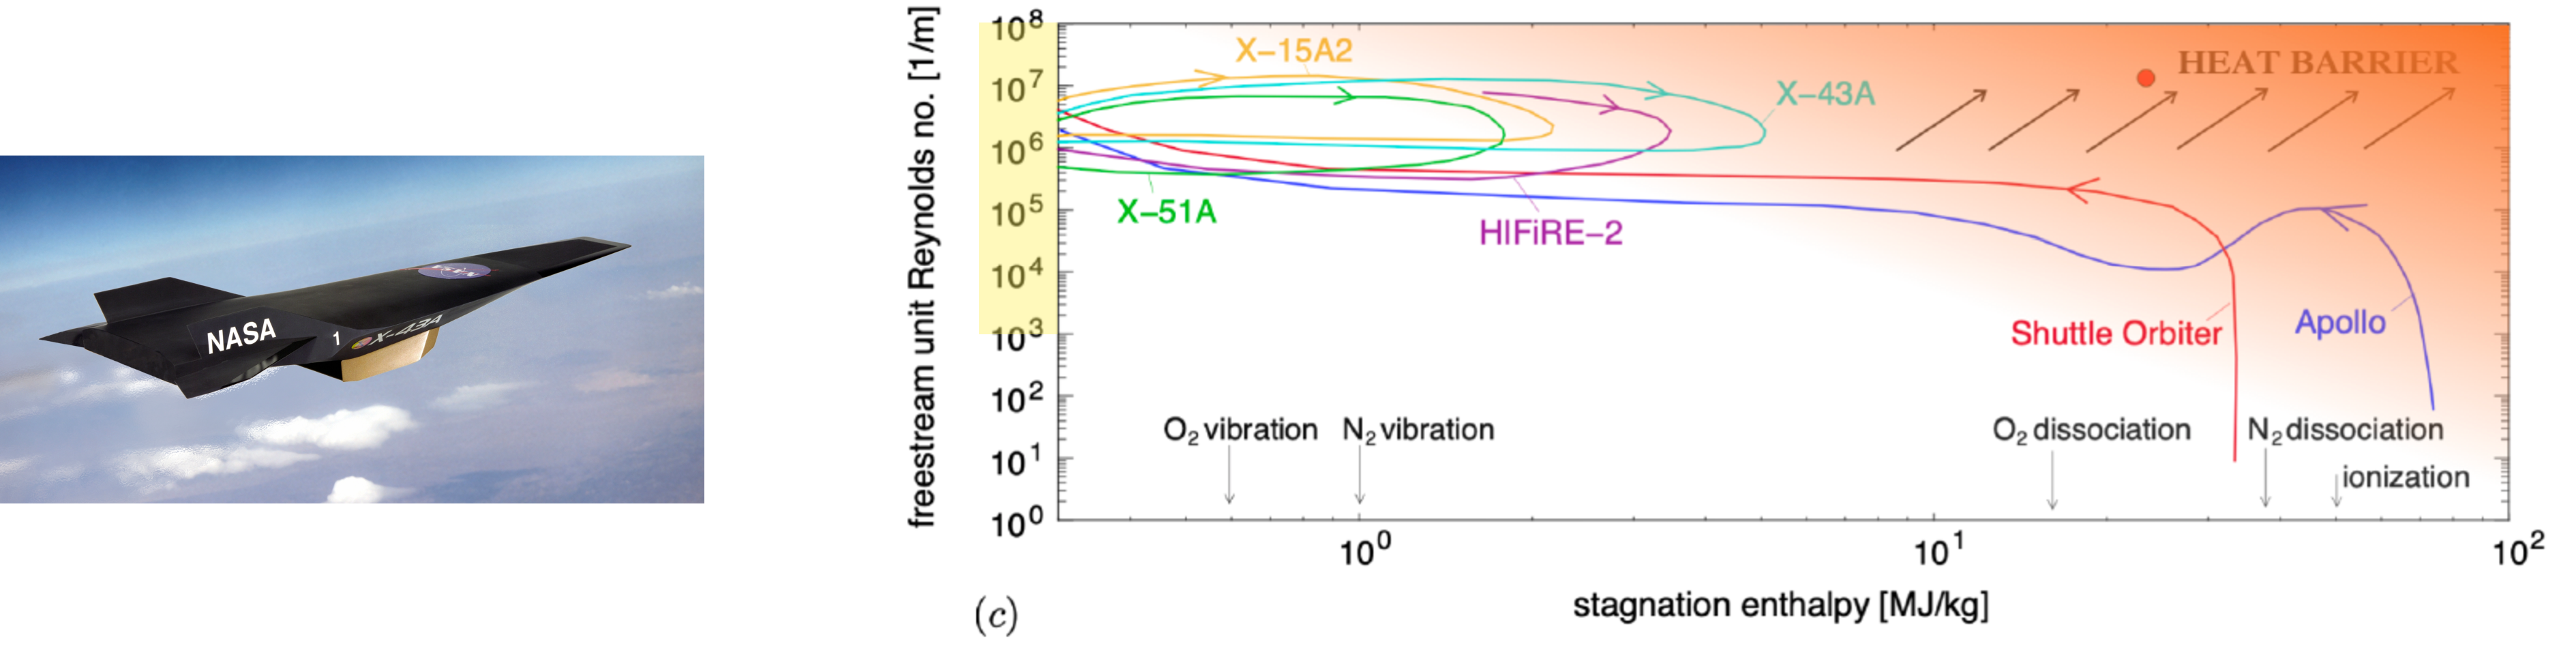
\includegraphics[scale=0.21]{figures/huete2021/intro_3.pdf}
\end{figure}
\vspace{-0.2cm}
\hspace{5cm} \scriptsize{Urzay, J., \& Di Renzo, M. (2021). Annual Research Briefs, Center for Turbulence Research, 7-32.}

\vspace{0.3cm}

\normalsize
Hypersonic flight \acl{at low altitudes} is characterized by:

\vspace{0.2cm}

\begin{tabular}{ll}
   \hspace{-0.2cm} \tabitem High free-stream Mach numbers $\mathcal{M} \geq 5$ & \hspace{-0.2cm} \acl{\tabitem \small large normal Mach numbers}\\
   \hspace{-0.2cm} \tabitem High free-stream and post-shock & \hspace{-0.2cm} \acl{\tabitem \small  turbulent boundary layers}\\
   \hspace{0.15cm} unit Reynolds numbers $Re \sim 10^7-10^9$ m\textsuperscript{-1} & \\
   \hspace{-0.2cm} \tabitem High stagnation enthalpies $h_0\sim 5-30$ MJ/kg & \hspace{-0.2cm} \acl{\tabitem \small much higher than the vibrational specific energies}\\
    & \hspace{0.15cm} \acl{\small of O$_2$ and N$_2$}\\
   \hspace{-0.2cm} \tabitem Small mean free paths $\lambda\sim 0.1~\mu$m & \hspace{-0.2cm} \acl{\tabitem \small  short vibrational relaxation distances}\\
\end{tabular}
\end{frame}
%%%%%%%%%%%%%%%%
\section{Base model for single diatomic species}
\begin{frame}{\large Base model for single diatomic species}


\begin{columns}[t]
    \begin{column}{.55\textwidth}
    
    \begin{figure}
        \centering
        \includegraphics[scale=0.2]{figures/huete2021/ideal_shock.pdf}
    \end{figure}
    \only<1-3>{
    \hspace{0.3cm} Integral conservation equations accross shock\\
    \hspace{0.3cm} waves in \acl{dissociating} gases
    \begin{equation*}
        \begin{aligned}
        \rho_1 u_1 &=\rho_2 u_2,\\
        \aclgreen{p_1} + \rho_1 u_1^2 &= \acl{p_2} +\rho_2 u_2^2,\\
        \aclgreen{e_1}+\aclgreen{p_1}/\rho_1 +u_1^2/2 &= \acl{e_2}+ \acl{p_2}/\rho_2 +u_2^2/2 + \acl{q_d},
        \end{aligned}
    \end{equation*}
    }
    \only<1>{
    \hspace{0.3cm} Upstream flow is sufficiently cold to be\\
    \hspace{0.3cm} approximated as 
    \aclgreen{
    \begin{equation*}
            e_1 = (5/2) R_{g, \mathrm{A}_2} T_1, \quad p_1 = \rho_1 R_{g, \mathrm{A}_2} T_1.
    \end{equation*}
    }
    }
    \only<2-3>{
    \acl{
    \begin{equation*}
        \begin{aligned}
            p_2 &= \rho_2 R_{g, \mathrm{A}_2} T_2(1 + \alpha), \quad q_d = \alpha R_{g, \mathrm{A}_2} \Theta_d, \\
            e_2 &=R_{g,\mathrm{A}_2} T_2 \left[3\alpha + (1-\alpha)\left(\dfrac{5}{2}+\dfrac{\Theta_v/T_2}{{\rm e}^{\Theta_v/T_2}-1}\right) \right],\\
            \dfrac{\alpha^2}{1-\alpha}&= \reved{G m \Theta_r\left(\dfrac{\pi m k_B}{\hbar^2}\right)^{\hspace{-0.1cm}3/2}}\dfrac{\sqrt{T_2}}{\rho_2}{\rm e}^{-\frac{\Theta_d}{T_2}}\left(1-{\rm e}^{-\frac{\Theta_v}{T_2}}\right),
        \end{aligned}
    \end{equation*}
    }
    }
    \end{column}%
    \begin{column}{.5\textwidth}%
    \begin{center}
        \only<1-3>{
        \includegraphics[scale=0.22]{figures/huete2021/Figure2_labels.pdf}
        }
    \end{center}
    \visible<2-3>{
        \hspace{0.4cm} where \acl{$\alpha$} is the \acl{degree of dissociation},\\
        \hspace{0.4cm} defined as the mass fraction of $\mathrm{A}$ atoms in\\
        \hspace{0.4cm} the reaction $\mathrm{A}_2\rightleftharpoons \mathrm{A}+ \mathrm{A},$ that must be\\
        \hspace{0.4cm} solved with the aid of the chemical\\
        \hspace{0.4cm} equilibrium condition.
        \vspace{0.15cm}
        }
    \end{column}%
    \only<3>{
        \begin{center}
            \begin{tikzpicture}[overlay]
                \node[draw, color=myorange, line width=0.4mm, fill=white] at (-7.3,-4.1) {\href{https://doi.org/10.1063/5.0059948}{\includegraphics[scale=0.4]{figures/huete2021/snapshot_huete2021.pdf}}};
            \end{tikzpicture}
        \end{center}
    }
\end{columns}
\end{frame}
%%%%%%%%%%%%%%%%
\section{Extension to multi- species mixture}
\begin{frame}{\normalsize Extension to multi-species mixture and considering electronic excitation and ionization}
\vspace{-0.5cm}
\begin{columns}[t]
    \begin{column}{.55\textwidth}
    
    \begin{center}
        \begin{tikzpicture}
            \node at (0.1,0) {\href{https://combustion-toolbox-website.readthedocs.io/}{\includegraphics[scale=0.5]{figures/aiaa2023/sketch_CT.pdf}}};
        \end{tikzpicture}
    \end{center}
    
    \hspace{0.3cm} Combustion Toolbox is used to solve the\\
    \hspace{0.3cm} Rankine-Hugoniot (RH) relations
    \begin{equation*}
        \begin{aligned}
        p_2/p_1 &= 1 - \rho_1 u_1^2/p_1 \left(\rho_1/\rho_2 - 1\right),\\
        h_2 &= h_1 + u_2^2/2\left[1- \left(\rho_1/\rho_2\right)^2\right].
        \end{aligned}
    \end{equation*}
    \hspace{0.3cm} These equations are supplemented with:
    \begin{itemize}
        \item the ideal-gas equation of state $p =\rho R_{g} T$,
        \item NASA-9 coefficient polynomials database to model the thermodynamic functions.
    \end{itemize}
    \hspace{0.3cm} Combustion Toolbox is in \acl{excellent agreement}\\
    \hspace{0.3cm} with NASA's CEA and CANTERA within SD-Toolbox.
    
    \end{column}%
    \begin{column}{.5\textwidth}%
    \begin{center}
        \only<1>{
        \begin{center}
            \begin{animategraphics}[autoplay,type=png,scale=0.18,loop]{20}{figures/combustion_toolbox/gui_CT/gui_CT-}{001}{553}
            \end{animategraphics}
        \end{center}
        }
        \only<2->{
        \includegraphics[scale=0.215]{figures/huete2021/Hugoniot_benchmarking_air_CT_log_reactions_labels.pdf}
        \begin{itemize}
            \item Region (I): frozen chemistry.
            \item Region (II): mainly O$_2$ dissociation and recombination.
            \item Region (III): mainly N$_2$ dissociation and recombination.
            \item Region (IV): mainly \acl{electronic excitation} and \acl{ionization}.
        \end{itemize}
        }
    \end{center}
    \end{column}%

\end{columns}

\end{frame}

%%%%%%%%%%%%%%%%
\begin{frame}{\normalsize Extension to multi-species mixture and considering electronic excitation and ionization}
    \setlength{\leftmargini}{0.5em}
    \begin{columns}[c]
        \begin{column}{.45\textwidth}%
        \vspace{-0.3cm}
        \begin{center}
            \includegraphics[scale=0.085]{figures/aiaa2023/sketch_thermo.pdf}
        \end{center}
        
        Endothermicity due to dissociation, vibrational excitation, electronic excitation and ionization does the following:
        \vspace{0.3cm}
        
        \begin{itemize}
            \item increases the mean post-shock density,
            \item decreases the mean post-shock velocity,
            % \item decreases the mean post-shock Mach number
            \item decreases the mean post-shock temperature,
            \item which implies an increase in the mean pre-shock velocity.
        \end{itemize}
        \end{column}%
        \begin{column}{.45\textwidth}
        \begin{center}
            \vspace{-0.3cm}\textbf{$\quad\quad\quad$Jump conditions}\\ \vspace{0.3cm}
            
            \includegraphics[scale=0.23]{figures/aiaa2023/RH_jump_AIAA2023_labels.pdf}
        \end{center}
        \end{column}%
    \end{columns}
\end{frame}
%%%%%%%%%%%%%%%%
\section{LIA of turbulence interacting with hypersonic shocks}
\begin{frame}[t]{\large LIA of turbulence interacting with hypersonic shocks}
Considering:
\begin{itemize}
    \item turbulence is comprised of small fluctuations (\acl{weak}),
    \item pre-shock turbulence is \acl{isotropic} (no privileged direction),
    \item turbulent field composed of the superposition of \acl{vortical} disturbances,
    % \item Kovasznay decomposition into vortical, entropic and acoustic modes.
\end{itemize}
We can solve this problem analytically by using  
\begin{itemize}
    \item linearized Rankine-Hugoniot relations,
    \item linearized Euler equations in the post-shock gas.
\end{itemize}
\setlength{\leftmargini}{2em}

\vspace{-1cm}
\begin{columns}[c]
    \begin{column}{.5\textwidth}%
    \begin{tikzpicture}[overlay]
          \node at (3.75, -1) {\includegraphics[scale=0.08]{figures/aiaa2023/sketch_turbulence_mod_2.pdf}};
    \end{tikzpicture}
    \end{column}%
    \begin{column}{.35\textwidth}

    \textbf{Limits of validity}

    \vspace{0.1cm}
    
    Assumptions standard LIA:
    \begin{enumerate}[(a)]
        \item rms$(u_\ell) \ll a_1$ and $a_2$,
        \item $\xi_s \ll \ell$,
        \item $ \ell/ u_\ell\ll \ell^2/\nu$.
    \end{enumerate}
    
    With thermochemical effects:
    \begin{enumerate}[(d)]
         \item $\ell_T\ll \ell$
    \end{enumerate}
    For a given $\ell$, this condition becomes increasingly more accurate as the  altitude decreases.
    
    \end{column}%
\end{columns}


\end{frame}
%%%%%%%%%%%%%%%%
\begin{frame}{\large LIA of turbulence interacting with hypersonic shocks: amplification of TKE}
\begin{columns}[c] 
    \begin{column}{.48\textwidth}%
    \vspace{-0.45cm}
    \begin{center}
        \vspace{-0.3cm}\textbf{$\quad$ Calorically perfect gas}\\ \vspace{0.3cm}
    \end{center}
     \includegraphics[width=1\textwidth]{figures/huete2021/sketch_tke_1.pdf}
    \end{column}%
    \begin{column}{.48\textwidth}
    \begin{center}
        \vspace{-0.3cm}\textbf{$\quad$ Vibrationally Excited, Dissociating Gas}\\ \vspace{0.3cm}
    \end{center}
    \includegraphics[width=1\textwidth]{figures/huete2021/sketch_tke_2.pdf}
    \end{column}%
\end{columns}
\vspace{0.3cm}
Conservation of tangential momentum dictates that the transverse velocity fluctuations should increase across the shock -- these are larger at hypersonic velocities because of the associated larger post-shock densities induced by endothermic thermochemical effects.
\end{frame}
%%%%%%%%%%%%%%%%
\begin{frame}{\large LIA of turbulence interacting with hypersonic shocks: integral formulas}
    \begin{columns}[c]
    \begin{column}{.4\textwidth}%
    \begin{center}
        \vspace{-0.3cm}\textbf{$\quad$Turbulent Kinetic Energy}\\ \vspace{0.3cm}
        
        \includegraphics[width=1.2\textwidth]{figures/aiaa2023/K3D_molarfraction_SFMC2022_labels.pdf}
    \end{center}
    \end{column}%
    \begin{column}{.45\textwidth}
    \begin{center}
        \vspace{-0.3cm}\textbf{$\quad$Turbulence intensity and Turbulent Reynolds number}\\ \vspace{0.3cm}
        
        \includegraphics[width=0.88\textwidth]{figures/aiaa2023/Ratios_AIAA2023_labels.pdf}
    \end{center}
    \end{column}%
\end{columns}
\vspace{0.3cm}
In contrast, the incorporation of dissociation, vibrational excitation (regions II, III, IV), electronic excitation (regions III, IV) and ionization (region IV) predicts larger kinetic energy and turbulence intensity amplification rates, along with an increase in the turbulent Reynolds number accross the shock.
\end{frame}
%%%%%%%%%%%%%%%%
\section{Flight altitude effects}
\begin{frame}{\large Flight altitude effects}

\begin{itemize}
    \item LIA with thermochemical effects demands $\ell_T / \ell_i \ll 1$
    \item \acl{$\ell_T$ varies with upstream conditions}, i.e., with altitude
    \item An increase of pre-shock Mach number decreases $\ell_T$
    \item An increase of altitude increases $\ell_T$ 
\end{itemize}

\begin{figure}
    \centering
    \includegraphics[width=0.85\textwidth]{figures/aiaa2023/K3D_molarfraction_AIAA2023_altitude_pressure_mod_slides.pdf}
    \begin{tikzpicture}[overlay]
        \node at (-2, 6.9) {\includegraphics[width=0.35\textwidth]{figures/aiaa2023/sketch_turbulence_nonequilibrium.pdf}};
    \end{tikzpicture}
\end{figure}

\end{frame}
%%%%%%%%%%%%%%%%
\section{Conclusions}
{\aauwavesbg%
\begin{frame}[plain]%
  \setbeamercolor{itemize item}{fg=white}
  \finalpage{
    \begin{tikzpicture}[overlay]
          \node at (-0.5, 1.6) {\color{mydblue}{\large Conclusions}};
    \end{tikzpicture}
    \noindent
    \begin{minipage}[t]{.65\textwidth}
    \raggedright
    \small
    \textbf{Key takeaways} \\
    \footnotesize
    \begin{itemize}
      \item The RH jump conditions have been computed using \href{https://github.com/AlbertoCuadra/combustion_toolbox}{\acll{Combustion Toolbox}$^*$}, an in-house thermochemical code capable of capturing high-temperature phenomena (dissociation, \acll{ionization}, and recombination).
      \item Qualitative picture remains intact compared with the theoretical results obtained in \href{https://doi.org/10.1063/5.0059948}{[Physics of Fluids, 33(8), 086111 (2021)]}, which only accounted for vibrational and dissociation effects of single-species diatomic gases.
      \item Multi-species effects reshape the TKE curve by rendering two maxima that fit fairly well within the O$_2$ and N$_2$ dissociation processes.
      \item \acll{\textbf{Thermochemical effects arising at hypersonic velocities appear to enhance turbulent fluctuations in the post-shock gas.}}
    \end{itemize}
    \end{minipage}
    % It is available via a open-source GPLv3 license \url{https://combustion-toolbox-website.readthedocs.io}
    \hfill
    \noindent
    \begin{minipage}[t][2.5cm][t]{.08\textwidth}
    \pagebreak
    \vspace{-0.1cm}
    \href{https://github.com/AlbertoCuadra/combustion_toolbox}{\includegraphics[scale=0.06]{figures/qr/qr_code_github.pdf}}
    \pagebreak
    \end{minipage}
    
    \begin{tikzpicture}[overlay]
          \node at (-1.5, -0.4) {\scriptsize $^*$ It is available under an open-source GPLv3 license via \url{https://combustion-toolbox-website.readthedocs.io}.};
          \node at (6.15, -0.41) { \href{mailto:acuadra@ing.uc3m.es}{\scriptsize acuadra@ing.uc3m.es}};
    \end{tikzpicture}
    }
    
\end{frame}}
%%%%%%%%%%%%%%%%
\section*{Supplementary material}
\begin{frame}{\large Supplementary material: monochromatic waves}
    \begin{columns}[t]
    \begin{column}{.465\textwidth}%
        
        \vspace{-0.3cm}
        The amplitude of the vorticity fluctuations
        \begin{equation*}
            \Omega = \begin{cases}
                 \Omega_{l} \quad &\text{if} \,\ \zeta \leq 1  \\
                 \Omega_{s} \quad &\text{if} \,\ \zeta \geq 1 \\
            \end{cases}
        \end{equation*}
        depends of the frequency parameter $\zeta$:
        \begin{itemize}
            \item long-wavelength regime \colorgreen{$\zeta < 1$}\\ (vortical mode)
            \item short-wavelength regime \colorred{$\zeta > 1$}\\ (vortical and  acoustic modes)
        \end{itemize}
        
        \includegraphics[width=0.8\textwidth]{figures/huete2021/vorticity_wave.pdf}
        
    \end{column}%
    \begin{column}{.5\textwidth}%
        \begin{center}
            \textbf{$\quad$Square of the vorticity amplitude}
        \end{center}
        
        \only<1>{
        \\ \vspace{0.3cm}
        \includegraphics[width=0.9\textwidth]{figures/huete2021/square_vorticity_log_colors_AIAA2023.pdf}
        }
        
        \\ \vspace{-0.4cm}
        \begin{figure}	
        	\color{black}
        	\begin{adjustbox}{max totalsize={0.95\textwidth}{0.95\textheight}}
        	    \only<2->{
        		\begin{tikzpicture}
        		\node[scale=1] (img) at (0,0) {\begin{animategraphics}[autoplay,method=ocg,label=comp1c,type=pdf,scale=1,loop]{10}{figures/huete2021/movie_monochromatic/dataW3D}{1}{99} 
            	\end{animategraphics}};
        		\end{tikzpicture}
        		}
        	\end{adjustbox}
        \end{figure}
        
        \vspace{-0.5cm}
    \end{column}%
\end{columns}
\vspace{0.3cm}

Anticipating that the pre-shock turbulence is isotropic, there is no privileged direction of the wavenumber vector $\bm{k}$, which allows transforming the 3D problem into a 2D one with a simple rotation of the reference frame.
\end{frame}
%%%%%%%%%%%%%%%%
\begin{frame}{\large Supplementary material: integral formulas}
    \begin{columns}[c]
    \begin{column}{.45\textwidth}%
    \begin{center}
        \vspace{0.01cm}\textbf{$\quad$Anisotropy}\\ \vspace{0.3cm}
        
        \includegraphics[width=1\textwidth]{figures/huete2021/Anisotropy_AIAA2023.pdf}
    \end{center}
    \end{column}%
    \begin{column}{.45\textwidth}
    \begin{center}
        \vspace{-0.3cm}\textbf{$\quad$Entropic prefactors of the post-shock density variance}\\ \vspace{0.3cm}
        
        \includegraphics[width=1\textwidth]{figures/huete2021/G3D_AIAA2023.pdf}
    \end{center}
    \end{column}%
\end{columns}
\vspace{0.3cm}
\end{frame}
%%%%%%%%%%%%%%%%
\begin{frame}{\large Supplementary material: theoretical results of previous work (Huete 2021)}
    \begin{columns}[c]
    \begin{column}{.4\textwidth}%
    \begin{center}
        \vspace{-0.3cm}\textbf{$\quad$Turbulent Kinetic Energy}\\ \vspace{0.3cm}
        
        \includegraphics[width=1.1\textwidth]{figures/huete2021/tke_2.pdf}
    \end{center}
    \end{column}%
    \begin{column}{.45\textwidth}
    \begin{center}
        \vspace{-0.3cm}\textbf{$\quad$Turbulence intensity and Turbulent Reynolds number}\\ \vspace{0.3cm}
        
        \includegraphics[width=1\textwidth]{figures/huete2021/Ratios_APS_alpha.pdf}
    \end{center}
    \end{column}%
\end{columns}
\vspace{0.3cm}
In contrast, the incorporation of dissociation and vibrational excitation predicts larger kinetic energy and turbulence intensity amplification rates, along with an increase in the turbulent Reynolds number accross the shock.
\end{frame}
%%%%%%%%%%%%%%%%
\end{document}
